\documentclass[../Ansoegning.tex]{subfiles}
%------------------- DOKUMENTER SAMLES --------------------------
\begin{document}                                % Dokumentet påbegyndes
\begin{center}
    \textbf{\LARGE{Dokumentation for dansk statsborgerskab}}\vspace{-3ex}
\end{center}

Følgende figure dokumenterer mit danske statsborgerskab, som jeg har opnået gennem normalisation:
\begin{figure}[H]
	\centering
	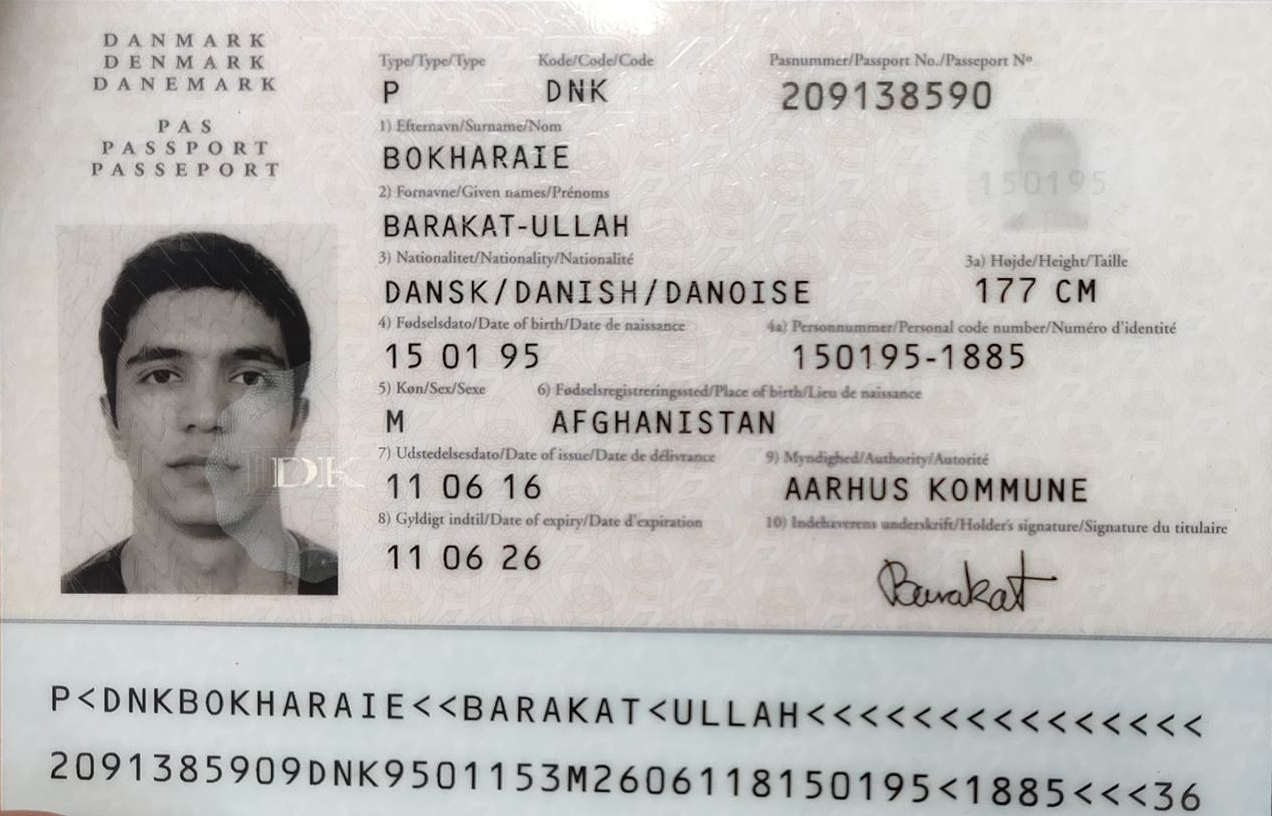
\includegraphics[width=0.87\textwidth]{Eksterne_filer/pas_ind.jpg}
\end{figure}

\begin{figure}[H]
	\centering
	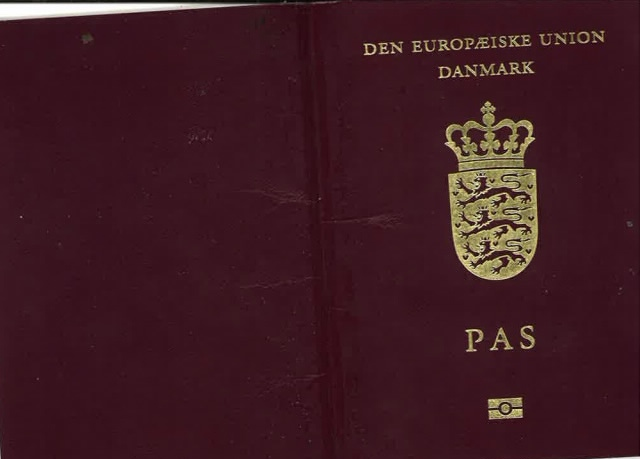
\includegraphics[width=0.87\textwidth]{Eksterne_filer/pas_for.jpg}
\end{figure}
\end{document}